An op amp having a low-frequency gain of $10^{3}$ and a single-pole rolloff at $10^{4}$ rad/s is connected in a negative feedback loop via a feedback network having a transmission $k$ and a two-pole rolloff at $10^{4}$ rad/s. Find the value of $k$ above which the closed-loop amplifier becomes unstable.
\begin{enumerate}[label=\arabic*.,ref=\theenumi]

%\begin{enumerate}[label=\thesection.\arabic*.,ref=\thesection.\theenumi]
\numberwithin{equation}{enumi}

\item Find the OPAMP gain $G(s)$.
\\
\solution 
The given oscillator has a low frequency gain $10^3$ and a single-pole rolloff at $10^4$ rad/s. So we have a open loop amplifier gain 
\begin{align}
G(s)&= \frac{10^3}{1+\frac{s}{10^4}}
\end{align}
\item Find the feedback $H(s)$
\\
\solution 
\begin{align}
H(s)&= \frac{k}{\left(1+\frac{s}{10^4}\right)^2}   
\end{align}
%
\item Find the  loop-gain $L(s)$. 
\\
\solution The loop gain is given by 
\begin{align}
L(s) = G(s)H(s) &= \frac{10^3k}{\left(1+\frac{s}{10^4}\right)^3}
\end{align}
and the various gains summarised in Table \ref{table:ee18btech11006_Factors}

\begin{table}[!ht]
\centering
%%  This section checks if we are begin input into another file or  %%
%%  the file will be compiled alone. First use a macro taken from   %%
%%  the TeXbook ex 7.7 (suggestion of Han-Wen Nienhuys).            %%
\def\ifundefined#1{\expandafter\ifx\csname#1\endcsname\relax}


%%  Check for the \def token for inputed files. If it is not        %%
%%  defined, the file will be processed as a standalone and the     %%
%%  preamble will be used.                                          %%
\ifundefined{inputGnumericTable}

%%  We must be able to close or not the document at the end.        %%
	\def\gnumericTableEnd{\end{document}}


%%%%%%%%%%%%%%%%%%%%%%%%%%%%%%%%%%%%%%%%%%%%%%%%%%%%%%%%%%%%%%%%%%%%%%
%%                                                                  %%
%%  This is the PREAMBLE. Change these values to get the right      %%
%%  paper size and other niceties.                                  %%
%%                                                                  %%
%%%%%%%%%%%%%%%%%%%%%%%%%%%%%%%%%%%%%%%%%%%%%%%%%%%%%%%%%%%%%%%%%%%%%%

	\documentclass[12pt%
			  %,landscape%
                    ]{report}
       \usepackage[latin1]{inputenc}
       \usepackage{fullpage}
       \usepackage{color}
       \usepackage{array}
       \usepackage{longtable}
       \usepackage{calc}
       \usepackage{multirow}
       \usepackage{hhline}
       \usepackage{ifthen}
%%  End of the preamble for the standalone. The next section is for %%
%%  documents which are included into other LaTeX2e files.          %%
\else

%%  We are not a stand alone document. For a regular table, we will %%
%%  have no preamble and only define the closing to mean nothing.   %%
    \def\gnumericTableEnd{}

%%  If we want landscape mode in an embedded document, comment out  %%
%%  the line above and uncomment the two below. The table will      %%
%%  begin on a new page and run in landscape mode.                  %%
%       \def\gnumericTableEnd{\end{landscape}}
%       \begin{landscape}


%%  End of the else clause for this file being \input.              %%
\fi

%%%%%%%%%%%%%%%%%%%%%%%%%%%%%%%%%%%%%%%%%%%%%%%%%%%%%%%%%%%%%%%%%%%%%%
%%                                                                  %%
%%  The rest is the gnumeric table, except for the closing          %%
%%  statement. Changes below will alter the table's appearance.     %%
%%                                                                  %%
%%%%%%%%%%%%%%%%%%%%%%%%%%%%%%%%%%%%%%%%%%%%%%%%%%%%%%%%%%%%%%%%%%%%%%

\providecommand{\gnumericmathit}[1]{#1} 
%%  Uncomment the next line if you would like your numbers to be in %%
%%  italics if they are italizised in the gnumeric table.           %%
%\renewcommand{\gnumericmathit}[1]{\mathit{#1}}
\providecommand{\gnumericPB}[1]%
{\let\gnumericTemp=\\#1\let\\=\gnumericTemp\hspace{0pt}}
 \ifundefined{gnumericTableWidthDefined}
        \newlength{\gnumericTableWidth}
        \newlength{\gnumericTableWidthComplete}
        \newlength{\gnumericMultiRowLength}
        \global\def\gnumericTableWidthDefined{}
 \fi
%% The following setting protects this code from babel shorthands.  %%
 \ifthenelse{\isundefined{\languageshorthands}}{}{\languageshorthands{english}}
%%  The default table format retains the relative column widths of  %%
%%  gnumeric. They can easily be changed to c, r or l. In that case %%
%%  you may want to comment out the next line and uncomment the one %%
%%  thereafter                                                      %%
\providecommand\gnumbox{\makebox[0pt]}
%%\providecommand\gnumbox[1][]{\makebox}

%% to adjust positions in multirow situations                       %%
\setlength{\bigstrutjot}{\jot}
\setlength{\extrarowheight}{\doublerulesep}

%%  The \setlongtables command keeps column widths the same across  %%
%%  pages. Simply comment out next line for varying column widths.  %%
\setlongtables

\setlength\gnumericTableWidth{%
	50pt+%
	50pt+%
	50pt+%
0pt}
\def\gumericNumCols{3}
\setlength\gnumericTableWidthComplete{\gnumericTableWidth+%
         \tabcolsep*\gumericNumCols*2+\arrayrulewidth*\gumericNumCols}
\ifthenelse{\lengthtest{\gnumericTableWidthComplete > \linewidth}}%
         {\def\gnumericScale{\ratio{\linewidth-%
                        \tabcolsep*\gumericNumCols*2-%
                        \arrayrulewidth*\gumericNumCols}%
{\gnumericTableWidth}}}%
{\def\gnumericScale{1}}

%%%%%%%%%%%%%%%%%%%%%%%%%%%%%%%%%%%%%%%%%%%%%%%%%%%%%%%%%%%%%%%%%%%%%%
%%                                                                  %%
%% The following are the widths of the various columns. We are      %%
%% defining them here because then they are easier to change.       %%
%% Depending on the cell formats we may use them more than once.    %%
%%                                                                  %%
%%%%%%%%%%%%%%%%%%%%%%%%%%%%%%%%%%%%%%%%%%%%%%%%%%%%%%%%%%%%%%%%%%%%%%

\ifthenelse{\isundefined{\gnumericColA}}{\newlength{\gnumericColA}}{}\settowidth{\gnumericColA}{\begin{tabular}{@{}p{50pt*\gnumericScale}@{}}x\end{tabular}}
\ifthenelse{\isundefined{\gnumericColB}}{\newlength{\gnumericColB}}{}\settowidth{\gnumericColB}{\begin{tabular}{@{}p{60pt*\gnumericScale}@{}}x\end{tabular}}
\ifthenelse{\isundefined{\gnumericColC}}{\newlength{\gnumericColC}}{}\settowidth{\gnumericColC}{\begin{tabular}{@{}p{60pt*\gnumericScale}@{}}x\end{tabular}}

\begin{tabular}[c]{%
	b{\gnumericColA}%
	b{\gnumericColB}%
	b{\gnumericColC}%
	}

%%%%%%%%%%%%%%%%%%%%%%%%%%%%%%%%%%%%%%%%%%%%%%%%%%%%%%%%%%%%%%%%%%%%%%
%%  The longtable options. (Caption, headers... see Goosens, p.124) %%
%	\caption{The Table Caption.}             \\	%
% \hline	% Across the top of the table.
%%  The rest of these options are table rows which are placed on    %%
%%  the first, last or every page. Use \multicolumn if you want.    %%

%%  Header for the first page.                                      %%
%	\multicolumn{3}{c}{The First Header} \\ \hline 
%	\multicolumn{1}{c}{colTag}	%Column 1
%	&\multicolumn{1}{c}{colTag}	%Column 2
%	&\multicolumn{1}{c}{colTag}	\\ \hline %Last column
%	\endfirsthead

%%  The running header definition.                                  %%
%	\hline
%	\multicolumn{3}{l}{\ldots\small\slshape continued} \\ \hline
%	\multicolumn{1}{c}{colTag}	%Column 1
%	&\multicolumn{1}{c}{colTag}	%Column 2
%	&\multicolumn{1}{c}{colTag}	\\ \hline %Last column
%	\endhead

%%  The running footer definition.                                  %%
%	\hline
%	\multicolumn{3}{r}{\small\slshape continued\ldots} \\
%	\endfoot

%%  The ending footer definition.                                   %%
%	\multicolumn{3}{c}{That's all folks} \\ \hline 
%	\endlastfoot
%%%%%%%%%%%%%%%%%%%%%%%%%%%%%%%%%%%%%%%%%%%%%%%%%%%%%%%%%%%%%%%%%%%%%%

\hhline{|-|-|-}
	 \multicolumn{1}{|p{\gnumericColA}|}%
	{\gnumericPB{\centering}\textbf{Parameters}}
	&\multicolumn{1}{p{\gnumericColB}|}%
	{\gnumericPB{\centering}\textbf{Definition}}
	&\multicolumn{1}{p{\gnumericColC}|}%
	{\gnumericPB{\centering}\textbf{For given question}}

	
\\


\hhline{|---|}
	 \multicolumn{1}{|p{\gnumericColA}|}%
	{\gnumericPB{\centering}{Open loop gain}}
	&\multicolumn{1}{p{\gnumericColB}|}%
	{\gnumericPB{\centering}G}
	&\multicolumn{1}{p{\gnumericColC}|}%
	{\gnumericPB{\centering}{$\frac{10^3}{1+ \frac{s}{10^4}}$}}

\\
\hhline{|---|}
	 \multicolumn{1}{|p{\gnumericColA}|}%
	{\gnumericPB{\centering}Feedback factor}
	&\multicolumn{1}{p{\gnumericColB}|}%
	{\gnumericPB{\centering}H}
	&\multicolumn{1}{p{\gnumericColC}|}%
	{\gnumericPB{\centering}{$\frac{k}{\left({1+\frac{s}{10^4}} \right)^2}$}}

\\
\hhline{|---|}
	 \multicolumn{1}{|p{\gnumericColA}|}%
	{\gnumericPB{\centering}Loop gain}
	&\multicolumn{1}{p{\gnumericColB}|}%
	{\gnumericPB{\centering}GH}
	&\multicolumn{1}{p{\gnumericColC}|}%
	{\gnumericPB{\centering}{$ {k\left(\frac{10}{1+\frac{s}{10^4}}\right)}^3$}}

\\
\hhline{|-|-|-|}
\end{tabular}

\ifthenelse{\isundefined{\languageshorthands}}{}{\languageshorthands{\languagename}}
\gnumericTableEnd

\caption{}
\label{table:ee18btech11006_Factors}
\end{table}
%\\
%The closed loop gain would be
%\begin{align}
%T(s)=\frac{G(s)}{1+G(s)H(s)}
%\end{align}
%Generalized condition for the system to be stable:
%\begin{align}
%T(j\omega)=\frac{G(j\omega)}{1+G(j\omega)H(j\omega)}
%\end{align}
%Loop gain, $L(j\omega)=G(j\omega)H(j\omega)$.
%\begin{align}
%L(j\omega)=\abs{{G(j\omega)H(j\omega)}}e^{j\phi(\omega)}
%\end{align}
%Let 
%\begin{align}
%\exp\cbrak{\j \phase{L\brak{\j \omega_{\pi}}}} = -1
%\end{align}
%Let the frequency at which phase angle $\phi(\omega)$ becomes $180^{\circ}$ be $\omega_{180}$. At $\omega = \omega_{180}$ , $L(j\omega)$ is a negative real number.
\item Find the PM and the condition for stability.
\\
\solution 
For stability, $PM > 0$
%\begin{itemize}
%    \item if $\abs{{G(j\omega_{180})H(j\omega_{180})}}$ $<$ 1,$T(j\omega_{180}) >$ 1 \\ $\implies$ 
%    system is stable.
%    \item if $\abs{{G(j\omega_{180})H(j\omega_{180})}}$ $=$ 1,$T(j\omega_{180}) = \infty $ \\ $\implies$
%    system is unstable.
%    \item if $\abs{{G(j\omega_{180})H(j\omega_{180})}}$ $>$ 1,$T(j\omega_{180}) <$ 1 \\ $\implies$ 
%    system is unstable.
%\end{itemize}
For the given system 
\begin{align}
\phase{L\brak{\j\omega_{180}}}   &= 180 \degree
%&=  \angle\frac{10^3k}{\left(1+\frac{j\omega}{10^4}\right)^3} 
\\
\implies     -3\tan^{-1}\brak{{\frac{\omega_{180}}{10^4}}} &= -180 \degree
\\
   \implies \omega_{180} &= \sqrt{3}\times 10^4 \, rad/s
\end{align}
The Loop gain at $\omega_{180}$ is $G(j\omega_{180})H(j\omega_{180})$.
 The system becomes unstable if 
\begin{align}
G(j\omega_{180})H(j\omega_{180})\geq 1 \\
\implies \abs{\frac{10^3k}{\left(1+\frac{j\omega}{10^4}\right)^3}} \geq 1\\
\abs{\frac{10^3k}{\left(1-\sqrt{3}j\right)^3} } \geq 1
\end{align}
\begin{align}
     \frac{10^3k}{\abs{\sqrt{1+{\sqrt{3}}^2}}} \geq 1\\
     \frac{10^3k}{8} \geq 1 \\
     \implies k \geq 0.008
\end{align}
Hence, the value of k above which the system becomes unstable is 0.008. 
\item Design the feedback circuit $H$. \\
\solution
\begin{align}
H(s)&=\frac{V_f}{V_0}= \frac{k}{\left(1+\frac{s}{10^4}\right)^2} = k\left({\frac{1}{1+\frac{2s}{10^4}+\frac{s^2}{10^8}}}\right)  
\end{align}
This is of the form,
\begin{align}
k\left(\frac{1}{1+s{R_1}{C_1}+{s^2}{L_1}{C_1}}\right) =  k\left(\frac{\frac{1}{s{C_1}}}{{R_1}+s{L_1}+\frac{1}{s{C_1}}}\right)  
\end{align}
This can be realized using the circuit,
\begin{figure}[!ht]
	\begin{center}
		\resizebox{\columnwidth}{!}{\begin{circuitikz}
\ctikzset{bipoles/length=1cm}

\draw 
(0, 0) node[op amp] (opamp) {}
(opamp.-) -- (-2,0.35)  node[ground]{}
(opamp.out) to[L =$L_1$,*-*] (2,0)to[R=$R_1$](4,0) to [C](4,-2.4) node[ground]{}
(opamp.+)   to (-1.8,-0.35)node at (-2,-0.35){$V_0$}
(opamp.center) node[]{k};
\draw node at (4.6,-1.2){$V_f$}
node at (4.6,0){$+$}
node at (4.6,-2.4){$-$}
node at (3.5,-1.2){$C_1$}
;\end{circuitikz}
}
	\end{center}
\caption{}
\label{fig:ee18btech11006_2}
\end{figure} \\
A set of values that satisfy these equations are,
\begin{align}
R_1&= 200\ohm \\
C_1&= 1\mu F\\
L_1&= 10mH 
\end{align}
\item Design the closed loop circuit.  You may choose a suitable vale of $k$ such that the system is stable.\\
\solution Let k=0.001. The closed loop gain is T(s).
\begin{align}
    T(s)&=\frac{\frac{10^3}{1+\frac{s}{10^4}}}{1+\frac{1}{\left(1+\frac{s}{10^4}\right)^3}}\\
    &=\frac{10^7s^2+2\times10^{11}s+10^{15}}{s^3+3\times10^4s^2+3\times10^8s+2\times10^{12}}
\end{align}
The final circuit would be:
\begin{figure}[!ht]
	\begin{center}
		\resizebox{\columnwidth}{!}{\begin{circuitikz}
\ctikzset{bipoles/length=1cm}
\draw 
(0, 0) node[op amp] (opamp) {}
(opamp.-) to (-1,0.35) node[ground]{}
(opamp.center) node{$k$}
(opamp.out) to [R=$R_1$](3,0) to [L=$L_1$](5,0) to [C=$C_1$](5,-3) node[ground]{};
\draw (7.5,-0.35) node[op amp] (opamp_1){}
(opamp_1.-) -- (5,0)
(opamp_1.+) to[V=$V_i$](6.7,-3) node[ground]{}
(opamp_1.center) node{$10^3$}
(opamp_1.out) to [L=$L_2$](10,-0.35) to [R=$R_2$](10,-3)node[ground]{}
(10,-0.35) -- (11,-0.35)--(11,-4)--(-0.8,-4)to (opamp.+)
(11,-0.35) to (11.5,-0.35)node at (11.8,-0.35){$V_0$}
(5,0)--(5,0.2)node at (5,0.5){$V_f$};
\end{circuitikz}
}
	\end{center}
\caption{}
\label{fig:ee18btech11006_6}
\end{figure}
\begin{align}
R_1&= 200\ohm \\
C_1&= 1\mu F\\
L_1&= 10mH \\
L_2&=1\mu F\\
R_2&=100\ohm\\
k&=10^{-3}
\end{align}
\item Sketch the Bode plot of the closed loop system
\solution The following code gives the Bode plot of the closed loop system
\begin{lstlisting}
codes/ee18btech11006/ee18btech11006_1.py
\end{lstlisting}
Bode Plot:
\begin{figure}[ht!]
\centering
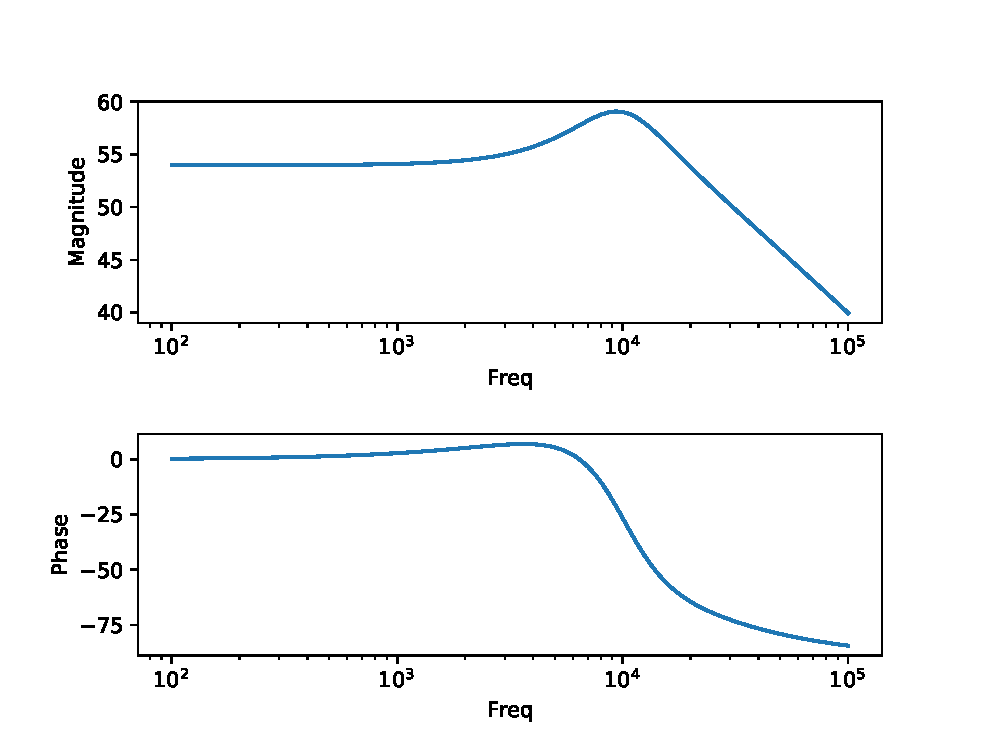
\includegraphics[width=\columnwidth]{./figs/ee18btech11006/ee18btech11006_7.eps}
\caption{}
\label{fig:ee18btech11006_7}
\end{figure}
\item Find the output of the circuit for an appropriate input using spice.\\
\solution
The following readme file provides necessary instructions to simulate the circuit in spice.
\begin{lstlisting}
codes/ee18btech11006/spice/README
\end{lstlisting}
The following netlist simulates the given circuit.
\begin{lstlisting}
codes/ee18btech11006/spice/ee18btech11006.net
\end{lstlisting}
The following code plots the output from the spice simulation which is shown in Fig. \ref{fig:ee18btech11006_8}.
\begin{lstlisting}
codes/ee18btech11006/spice/ee18btech11006_spice.py
\end{lstlisting}
\renewcommand{\thefigure}{\theenumi.\arabic{figure}}
%
\begin{figure}[!ht]
\centering
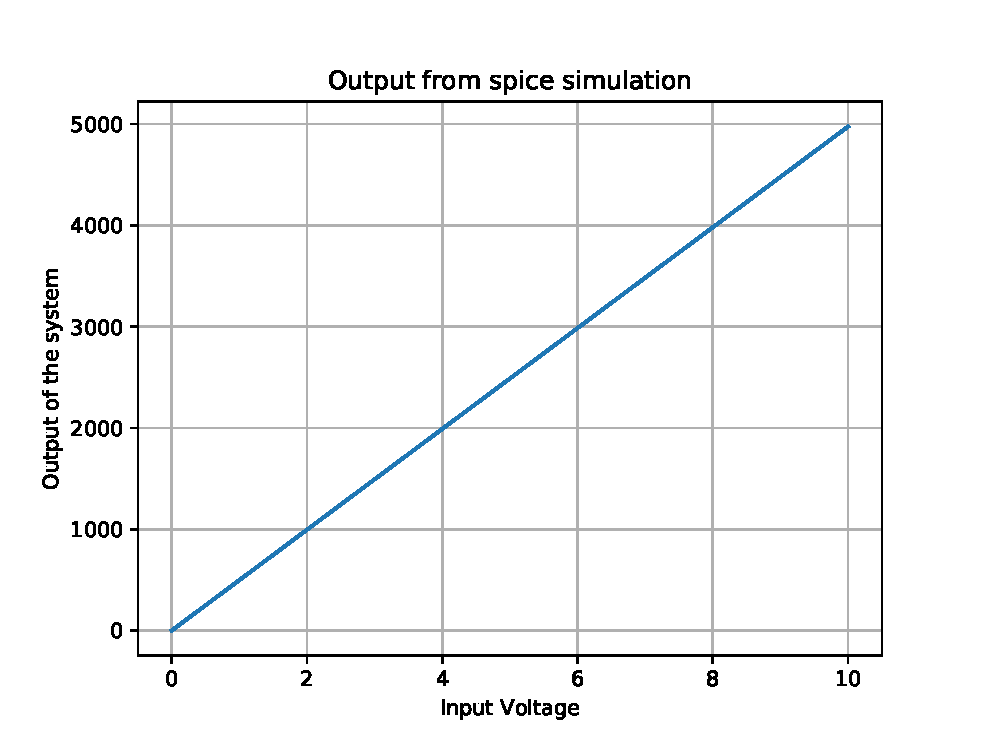
\includegraphics[width=\columnwidth]{./figs/ee18btech11006/ee18btech11006_8.eps}
\caption{}
\label{fig:ee18btech11006_8}
\end{figure}
\textbf{Verification}: The Output of the system would be :
\begin{align}
    Y(s)&=T(s)X(s)\\
    X(s)&=\frac{A}{s}\\
    Y(s)&=A\frac{10^7s^2+2\times10^{11}s+10^{15}}{s^4+3\times10^4s^3+3\times10^8s^2+2\times10^{12}s}
\end{align}
The following python codes plot the inverse Laplace of Y(s) giving the time domain output for different values of A.
\begin{lstlisting}
codes/ee18btech11006/spice/ee18btech11006_2.py
\end{lstlisting}
On plotting, we obtain the given figure.\\
\begin{figure}[!ht]
\centering
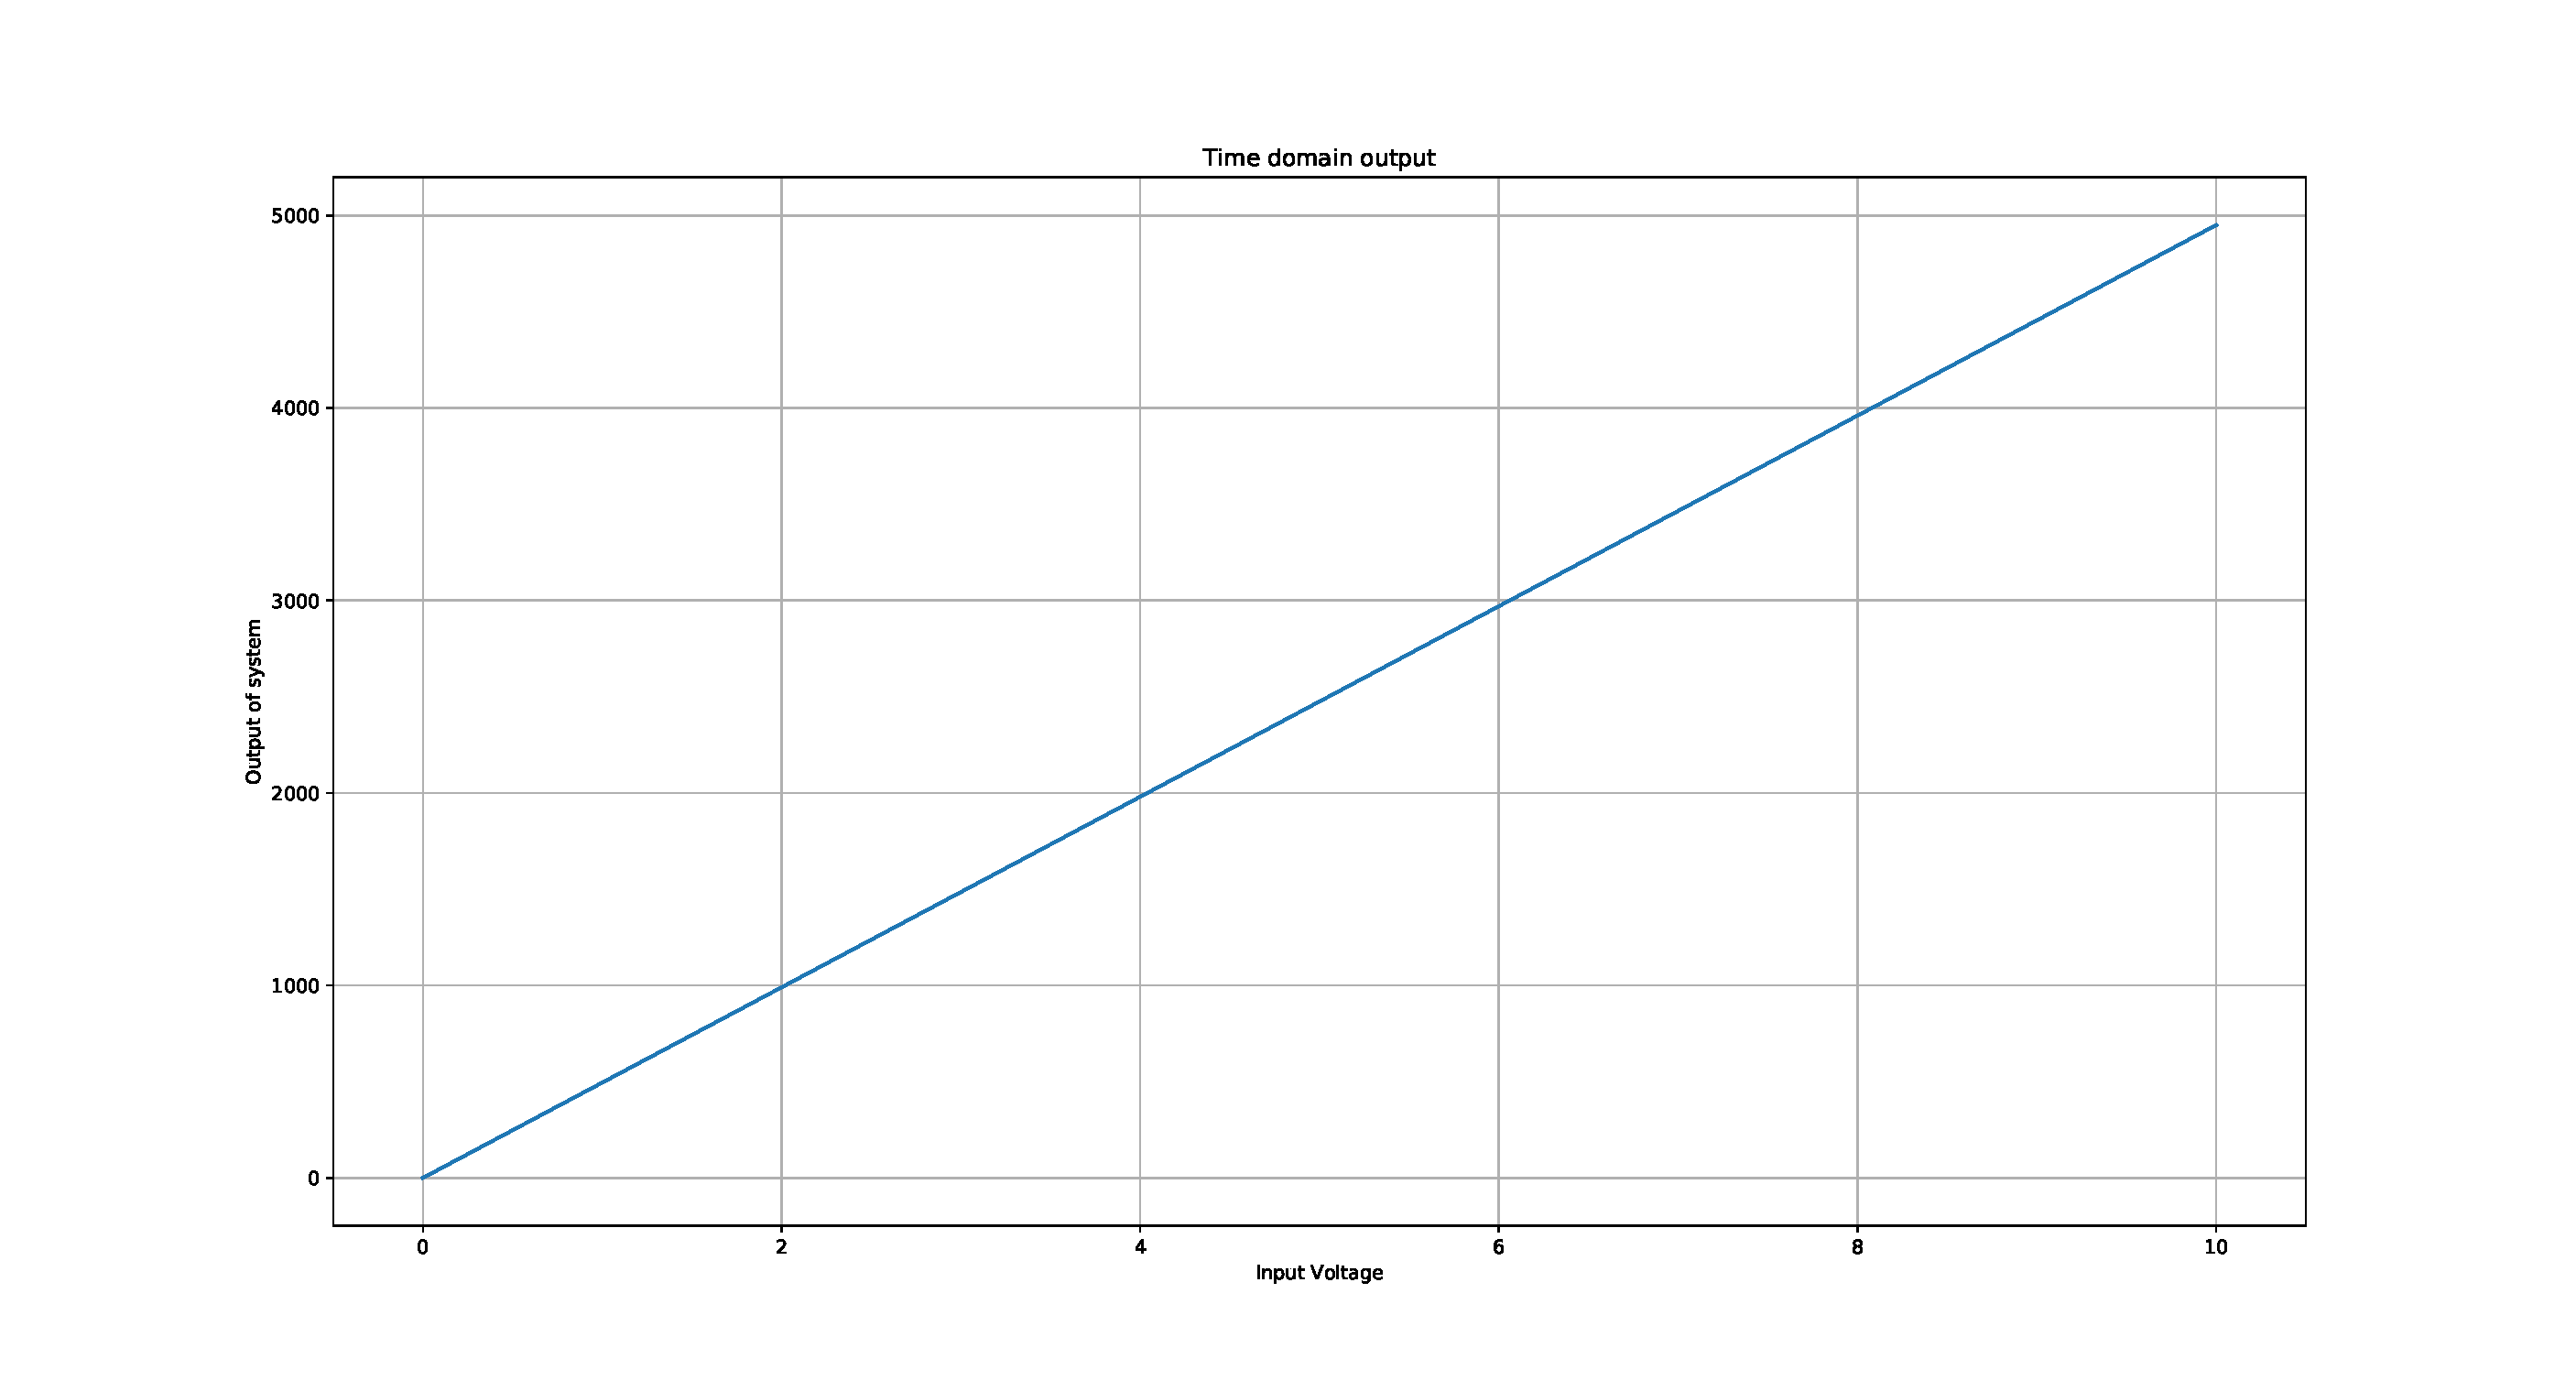
\includegraphics[width=\columnwidth]{./figs/ee18btech11006/ee18btech11006_9.eps}
\caption{}
\label{fig:ee18btech11006_9}
\end{figure}
Hence verified that the designed circuit does represent the given system.
\end{enumerate}

